% Paquets généraux
\documentclass[a4paper,12pt,titlepage]{article}
\usepackage[T1]{fontenc}
\usepackage[utf8]{inputenc}
\usepackage[french]{babel}
\usepackage[gen]{eurosym}
%\usepackage[dvips]{graphicx}
\usepackage{fancyhdr}
\usepackage{pdfpages} 
\usepackage{multido}
\usepackage{moreverb}
\usepackage{hyperref}
%\usepackage{textcomp}
\usepackage{verbatim}
\usepackage{moreverb}
\usepackage{listings}
\usepackage{minted}
\usepackage{eso-pic}
\usepackage{enumitem}
\usepackage{comment}
\usepackage{boxedminipage}
\usepackage[french,onelanguage, boxruled,linesnumbered]{algorithm2e}


\newcommand{\auteurun}{Juliette Genzmer}
\newcommand{\auteurdeux}{Willie Robert}
\newcommand{\auteurtrois}{Renaud Costadoat}
\newcommand{\institute}{Lycée Dorian}
\newtheorem{solution}{Solution}


\newcommand{\nom}{Porte conteneur}
\newcommand{\sequence}{03}
\newcommand{\num}{04}
\newcommand{\type}{TD}
\newcommand{\descrip}{Résolution d'un problème en utilisant des méthodes algorithmiques}
\newcommand{\competences}{Alt-C3: Concevoir un algorithme répondant à un problème précisément posé}

\usepackage{color}
\usepackage{xcolor}
\usepackage{colortbl}
\usepackage{helvet}
\renewcommand{\familydefault}{\sfdefault}
\usepackage{amsfonts}
\usepackage{amsmath}
%\usepackage{xspace}
\usepackage{varioref}
\usepackage{tabularx}
%\usepackage{floatflt}
\usepackage{graphics}
\usepackage{wrapfig}
\usepackage{textcomp}
\usepackage{tikz}
\usepackage{wrapfig}
\usepackage{gensymb}
\usepackage{ifthen}
\usepackage{cancel}
\usepackage{etoolbox}
\usepackage{multirow}
%\usepackage{boxedminipage}
\definecolor{gris25}{gray}{0.75}
\definecolor{bleu}{RGB}{18,33,98}
\definecolor{bleuf}{RGB}{42,94,171}
\definecolor{bleuc}{RGB}{231,239,247}
\definecolor{rougef}{RGB}{185,18,27}
\definecolor{rougec}{RGB}{255,188,204}%255,230,231
\definecolor{vertf}{RGB}{103,126,82}
\definecolor{vertc}{RGB}{220,255,191}
\definecolor{forestgreen}{rgb}{0.13,0.54,0.13}
\definecolor{blcr}{rgb}{0.59,0.69,0.84}
\definecolor{blfr}{rgb}{0.32,0.51,0.75}
\definecolor{orfr}{rgb}{0.90,0.42,0.15}
\definecolor{orcr}{rgb}{0.90,0.65,0.50}
\definecolor{orangef}{rgb}{0.659,0.269,0.072}
\definecolor{orange}{rgb}{0.58,0.35,0.063}
\definecolor{orangec}{rgb}{0.43,0.32,0.25}
\definecolor{rcorrect}{rgb}{0.6,0,0}
\definecolor{sequence}{rgb}{0.75,0.75,0.75}
\definecolor{competences}{rgb}{0.61,0.73,0.35}
\definecolor{grisf}{HTML}{222222}
\definecolor{grisc}{HTML}{636363}
\definecolor{normal}{HTML}{4087c4}
\definecolor{info}{HTML}{5bc0de}
\definecolor{success}{RGB}{92,184,92}
\definecolor{warning}{RGB}{240,173,78}
\definecolor{danger}{RGB}{217,83,79}
\hypersetup{                    % parametrage des hyperliens
    colorlinks=true,                % colorise les liens
    breaklinks=true,                % permet les retours à la ligne pour les liens trop longs
    urlcolor= blfr,                 % couleur des hyperliens
    linkcolor= orange,                % couleur des liens internes aux documents (index, figures, tableaux, equations,...)
    citecolor= forestgreen                % couleur des liens vers les references bibliographiques
    }

% Mise en page
\pagestyle{fancy}

\setlength{\hoffset}{-18pt}

\setlength{\oddsidemargin}{0pt} 	% Marge gauche sur pages impaires
\setlength{\evensidemargin}{0pt} 	% Marge gauche sur pages paires
\setlength{\marginparwidth}{00pt} 	% Largeur de note dans la marge
\setlength{\headwidth}{481pt} 	 	% Largeur de la zone de tête (17cm)
\setlength{\textwidth}{481pt} 	 	% Largeur de la zone de texte (17cm)
\setlength{\voffset}{-18pt} 		% Bon pour DOS
\setlength{\marginparsep}{7pt}	 	% Séparation de la marge
\setlength{\topmargin}{-30pt} 		% Pas de marge en haut
\setlength{\headheight}{55pt} 		% Haut de page
\setlength{\headsep}{20pt} 		% Entre le haut de page et le texte
\setlength{\footskip}{30pt} 		% Bas de page + séparation
\setlength{\textheight}{700pt} 		% Hauteur de l'icone zone de texte (25cm)
\setlength\fboxrule{1 pt}
\renewcommand{\baselinestretch}{1}
\setcounter{tocdepth}{1}
\newcommand{\cadre}[2]
{\fbox{
  \begin{minipage}{#1\linewidth}
   \begin{center}
    #2\\
   \end{center}
  \end{minipage}
 }
}

\newcounter{num_quest} \setcounter{num_quest}{0}
\newcounter{num_rep} \setcounter{num_rep}{0}
\newcounter{num_cor} \setcounter{num_cor}{0}

\newcommand{\question}[1]{\refstepcounter{num_quest}\par
~\ \\ \parbox[t][][t]{0.15\linewidth}{\textbf{Question \arabic{num_quest}}}\parbox[t][][t]{0.85\linewidth}{#1\label{q\the\value{num_quest}}}\par\par
}



\newcommand{\reponse}[0]{\refstepcounter{num_rep}\par
~\ \\ \parbox[t][][t]{0.15\linewidth}{\textbf{Question \arabic{num_rep}}}}

\newcommand{\cor}
{\refstepcounter{num_cor}
\noindent
\rule{\linewidth}{.5pt}
\textbf{Question \arabic{num_cor}:} \\
}



% En tête et pied de page
\lhead{\nom}
\rhead{
\includegraphics[width=2cm]{../../../img/logo}}
\lfoot{David Aubert, Renaud Costadoat}
\rfoot{Page \thepage}
\cfoot{}

\newlength{\RoundedBoxWidth}
\newsavebox{\GrayRoundedBox}
\newenvironment{GrayBox}[1][\dimexpr\textwidth-4.5ex]%
   {\setlength{\RoundedBoxWidth}{\dimexpr#1}
    \begin{lrbox}{\GrayRoundedBox}
       \begin{minipage}{\RoundedBoxWidth}}%
   {   \end{minipage}
    \end{lrbox}
    \begin{center}
    \begin{tikzpicture}%
       \draw node[draw=bleuf,fill=bleuc,rounded corners,%
             inner sep=2ex,text width=\RoundedBoxWidth]%
             {\usebox{\GrayRoundedBox}};
    \end{tikzpicture}
    \end{center}}

\fancypagestyle{correction}{%
  \fancyhf{}
  \lhead{\colorbox{danger}{\begin{minipage}{0.65\paperwidth} \textcolor{white}{\textbf{Correction}} \end{minipage}} }
  \rhead{
\includegraphics[width=2cm]{../../../img/logo}}
  \lfoot{Juliette Genzmer, Willie Robert, Renaud Costadoat}
  \rfoot{\colorbox{danger}{\begin{minipage}{0.3\paperwidth} \begin{flushright}\textcolor{white}{\textbf{Correction}}\end{flushright} \end{minipage}} }}

\renewcommand{\footrulewidth}{0.4pt}


\newcommand{\BackgroundPic}{%
\put(0,0){%
\parbox[b][\paperheight]{\paperwidth}{%
\vfill
\begin{center}
\hspace{0.5cm}\vspace{0.5cm}

\includegraphics[width=\paperwidth,height=\paperheight,%
keepaspectratio]{../../../img/fond5}%
\end{center}
\vfill
}}}

\newcommand{\goforum}{
\begin{figure}[ht!]
\begin{center}
 
\includegraphics[width=0.7\linewidth]{../../../img/go_forum}
\end{center}
\label{go_forum}
\caption{J'pète les plombs}
\end{figure}}

\newcommand{\BackgroundPicdeux}{%
\put(25,-30){%
\parbox[b][\paperheight]{\paperwidth}{%
\vfill
\begin{center}

\includegraphics[width=\paperwidth,height=\paperheight,%
keepaspectratio]{../../../img/fond6}%
\end{center}
\vfill
}}}

\setenumerate[1]{align=left,label=\arabic*}
\setenumerate[2]{before=\stepcounter{enumi},label*=.\arabic*,leftmargin=1.2em,align=left}

\begin{document}


\pagestyle{fancy}

\AddToShipoutPicture{\BackgroundPicdeux}

\section{Introduction}

\question{Ecrire sur le diagramme de Contexte donné en document réponse le nom des composants de l'unité centrale.}

\section{Analyse d'une réponse temporelle}

Le tracé de la figure \ref{fig01} correspond à la réponse $s(t)$ à un échelon $u(t)=1$ de la fonction de transfert $H(p)$, avec:

\begin{center}
$H(p)=\frac{K}{1+\frac{2.\xi}{\omega_0}.p+\frac{p^2}{\omega_0^2}}$
\end{center}

\vspace{-1cm}

\begin{figure}[!ht]
\centering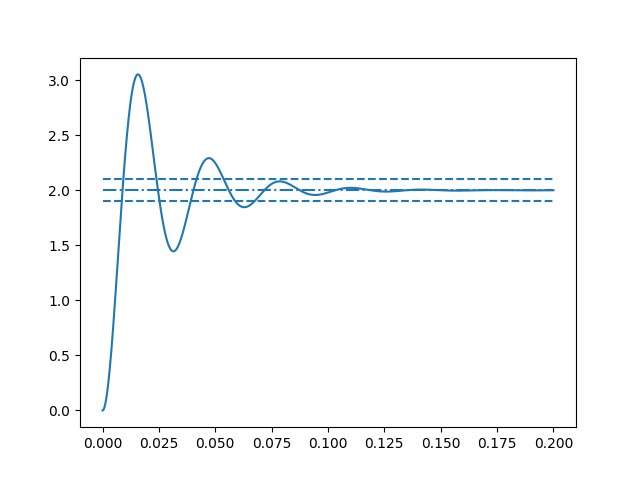
\includegraphics[width=0.7\linewidth]{img/fig01}
\caption{Tracé de la réponse temporelle s(t)}
\label{fig01}
\end{figure}

Sont indiquées sur la figure l'asymptote à la courbe quand $t$ tend vers l'infini (en trait mixte) et les droites limites à $+/-5\%$ de cette asymptote (en pointillés).

L'objectif de cette étude est d'écrire un script python permettant d'identifier les paramètres $\xi$, $\omega_0$ et $K$ de cette fonction de transfert.

Afin d'effectuer ce tracé, deux listes ont été créées:
\begin{itemize}
 \item \verb?t? contenant l'ensemble des valeurs de $t$,
 \item \verb?s? contenant l'ensemble des valeurs de $s(t)$.
\end{itemize}

Rappel: \verb? L[-1]? donne la dernière valeur de la liste \verb?L?.

\question{Ecrire sous python la commande permettant de déterminer $K$ à partir de \verb?s?.}

~\

On donne la fonction python \verb?recherche(s)? ci-dessous qui recherche la valeur \verb?val? dans la liste \verb?s?.

\begin{center}
\begin{minted}[frame=lines]{python}
def recherche(s):
    val=s[0]
    for i in range(len(s)):
        if s[i] > val:
            val=s[i]
    return val
\end{minted}
\end{center}

\question{Préciser quelle est la particularité de cette valeur \verb?val? pour la liste \verb?s?.}

\question{Justifier que le code suivant permet de calculer \verb?Tp? la valeur de la pseudo période de $s(t)$.}
\begin{center}
\begin{minted}[frame=lines]{python}
i=0
while s[i]!=recherche(s):
    i+=1
Tp=2*t[i]
\end{minted}
\end{center}

On rappelle que le dépassement en pourcent défini comme suit: $D_\%=100.\frac{s(max)-s(+\infty)}{s(+\infty)}$ peut être calculé en fonction de $\xi$ comme suit $D_\%=100.e^{-\frac{\xi.\pi}{\sqrt{1-\xi^2}}}$, on a donc défini la fonction \verb?D(xi)? suivante:

\begin{center}
\begin{minted}[frame=lines]{python}
def D(xi):
    return 100*np.exp(-xi*np.pi/np.sqrt(1-xi**2))
\end{minted}
\end{center}

Afin de rechercher la valeur de $\xi$, on propose de suivre l'algorithme suivant:
\begin{enumerate}
 \item On sait que $\xi<0.7$ car il y a un dépassement au dessus de la droite à $+5\%$, donc on démarre avec \verb?xi=0.7?,
 \item On regarde si \verb?D(xi)? est plus petit que $D_\%=100.\frac{s(max)-s(+\infty)}{s(+\infty)}$,
 \item Tant que c'est vrai, cela signifie que le $\xi$ est inférieur à \verb?xi?, alors on retire $0.01$ à \verb?xi?,
 \item Quand ce n'est plus vrai, cela signifie qu'on vient de trouver $\xi$.
\end{enumerate}

\question{Compléter le code python suivant afin de déterminer $\xi$ à partir des résultats précédents.}

\begin{center}
\begin{minted}[frame=lines]{python}
xi=0.7
while .........................................:
    xi+=-0.01
\end{minted}
\end{center}

On rappelle que $Tp=\frac{2.\pi}{\omega_0.\sqrt{1-\xi^2}}$

\question{Ecrire le code python permettant de déterminer $\omega_0$ à partir des résultats précédents.}

~\

Afin de vérifier nos résultats, nous souhaitons calculer le temps de réponse par deux moyens.

Dans un premier temps, nous allons chercher à le calculer à partir de \verb?s? en cherchant, en partant de la fin, le moment à partir duquel la valeur de $s(t)$ sort de la bande de $+/-5\%$. On donne pour cela l'extrait de code suivant:

\begin{center}
\begin{minted}[frame=lines]{python}
i=-1
while ...............................:
    i+=-1
t5=t[i+1]
\end{minted}
\end{center}

\question{Compléter le code afin d'obtenir le résultat souhaité.}

~\

On rappelle que $t_{R,5\%}=\frac{1}{\xi.\omega_0}.\ln(20)$, on donne donc la fonction suivante (\verb?log? correspond bien au logarithme népérien en python): 

\begin{center}
\begin{minted}[frame=lines]{python}
def tr5(xi,w0):
    return np.log(20)/(xi*w0)
\end{minted}
\end{center}
    
\question{Ecrire un code python qui affiche "OK" si la différence entre les deux valeurs calculées pour le temps de réponse est inférieure à 0,01s et "KO" si ce n'est pas le cas. La fonction valeur absolue s'écrit \verb?abs()? en python.}

\question{Expliquer l'intérêt du code suivant.}

{\scriptsize
\begin{center}
\begin{minted}[frame=lines]{python}
while t5>0.025:
    xi+=10**(-3)
    s=K*(1-np.exp(-w0*xi*t)/np.sqrt(1-xi**2)*np.cos(w0*np.sqrt(1-xi**2)*t-np.arctan(xi/np.sqrt(1-xi**2))))
    i=-1
    while s[i]<1.05*s[-1] and s[i]>0.95*s[-1]:
        i+=-1
    t5=t[i+1]
\end{minted}
\end{center}}


\section{Valeur approchée de $\xi$}

Il se trouve que le cahier des charges du système demande un temps de réponse à 5\% inférieur à 0,025s. Pour cela, il faut que $\xi$ soit environ égal à 0,65. Ce nombre doit alors stocké.

\question{Ecrire sous la forme d'un mot de 32 bits respectant la norme IEEE 754 (signe, exposant, mantisse) le float $0,65$.}

\question{Montrer que $00110011001100110011=\frac{2^{20}-1}{5}.$}

~\

On donne: $2^{-3}=0.125$, $2^{-1}=0.5$, $2^{-23}\approx 1,2.10^{-7}$.

\question{Déterminer l'erreur due au stockage de 0,65 à l'aide de la norme IEE74.}

\newpage

\section{Document réponse}

Nom:.....................\\
Prénom:......................

\begin{center}
 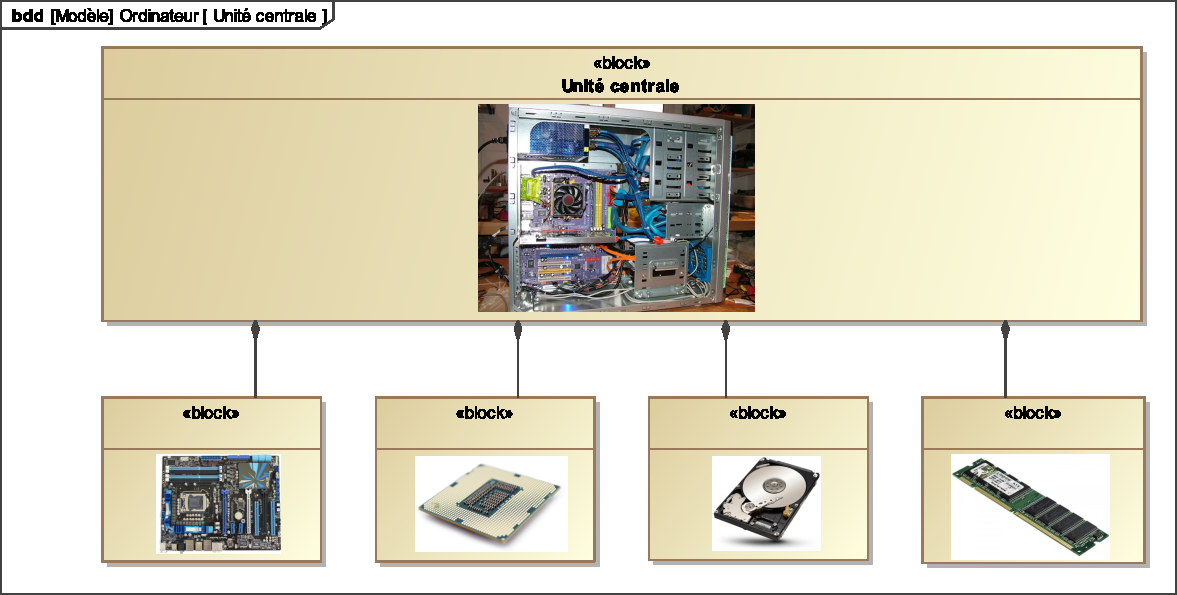
\includegraphics[width=0.9\linewidth]{img/unite_centrale_vierge}
\end{center}

\ifdef{\public}{\end{document}}{}

\newpage

~\

\newpage
\cleardoublepage

\pagestyle{correction}\setcounter{section}{0}

\section{Correction}

\paragraph{Question 1:}

\begin{center}
 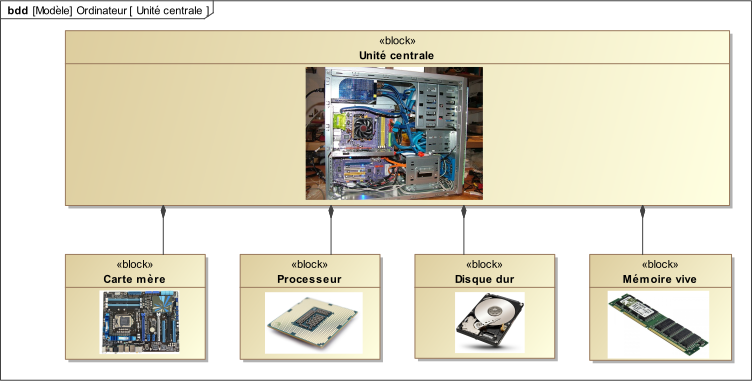
\includegraphics[width=0.9\linewidth]{img/unite_centrale_corrige}
\end{center}

\paragraph{Question 2:}

\verb?K=s[-1]?.

\paragraph{Question 3:}

La valeur \verb?val? est la plus grande valeur de la liste \verb?s?.

\paragraph{Question 4:}

Cette fonction cherche le temps qui correspond au double du temps correspondant au point le plus haut de la courbe. C'est bien $Tp$.

\paragraph{Question 5:}

\begin{center}
\begin{minted}[frame=lines]{python}
xi=0.7
while D(xi)<100*(recherche(s)-s[-1])/s[-1]:
    xi+=-0.01
\end{minted}
\end{center}

\paragraph{Question 6:}

\begin{center}
\begin{minted}[frame=lines]{python}
w0=2*np.pi/(Tp*np.sqrt(1-xi**2)
\end{minted}
\end{center}

\paragraph{Question 7:}


\begin{center}
\begin{minted}[frame=lines]{python}
i=-1
while s[i]<1.05*s[-1] and s[i]>0.95*s[-1]:
    i+=-1
t5=t[i+1]
\end{minted}
\end{center}

\paragraph{Question 8:}

\begin{center}
\begin{minted}[frame=lines]{python}
if abs(t5-tr5(xi,w0))<0.01:
    print("OK")
else:
    print("KO")
\end{minted}
\end{center}

\paragraph{Question 9:}

Le code suivant chercher la valeur de $\xi$ telle que le temps de réponse soit inférieur à 0,025s.

\paragraph{Question 10:}

Le nombre à traduire est $0,65_2$.

\begin{tabular}{c c c c c c c c c c}
0,65 & x & 2 & = & 1,3 & = &  1 & + & 0,3 \\
0,3 & x & 2 & = & 0,6 & = &  0 & + & 0,6 \\
0,6 & x & 2 & = & 1,2 & = &  1 & + & 0,2 \\
0,2 & x & 2 & = & 0,4 & = &  0 & + & 0,4 \\
0,4 & x & 2 & = & 0,8 & = &  0 & + & 0,8 \\
0,8 & x & 2 & = & 1,6 & = &  1 & + & 0,6 \\
0,6 & x & 2 & = & 1,2 & = &  1 & + & 0,2 \\
...
\end{tabular}

On remarque un récurrence dans l'écriture du $0,65_{10}$ en binaire: $0,65_{10}=0,10100110011.._2$

Le nombre stocké est alors:
$1,\underbrace{01001100110011001100110_2}_{23 bits}*2^{-1}$

\begin{itemize}
 \item Signe = $0$,
 \item Mantisse:$\underbrace{01001100110011001100110_2}_{23 bits}$,
 \item Exposant:$127-1=126_{10}=01111110_2$
\end{itemize}

\paragraph{Question 11:}

$a=00110011001100110011=11111111111111111111-11001100110011001100=
(2^{20}-1)-4*a$, donc $a=\frac{2^{20}-1}{5}$.

\paragraph{Question 12:}

Le nombre stocké est donc: $10100110011001100110011.2^{-23}=(2^{20}+2^{22}+\frac{2^{20}-1}{5}).2^{-23}=2^{-3}+2^{-1}+\frac{2^{-3}}{5}-\frac{2^{-23}}{5}=0,125+0,5+0,025-\frac{1,2.10^{-7}}{5}=0,65-24.10^{-9}$.

L'erreur est donc de $-\frac{1,2.10^{-7}}{5}=-24.10^{-9}$

\end{document}
